%\documentclass[t,10pt]{beamer}
\documentclass[t,handout]{beamer}

\usepackage{graphicx}
\usepackage{epsfig}
\usepackage{psfrag}
\usepackage[english]{babel}
\usepackage{color}
\usepackage{natbib}

%Mathematics packages
\usepackage{amsmath}
\usepackage{mathrsfs}
\usepackage{amsfonts}
\usepackage{enumerate}

\graphicspath{{./images/}} % Figures path - used in graphicx

\selectcolormodel{cmyk}

\mode<presentation>

%THEMES - Please refer to these chapters in the beamer documentation.
% Presentation themes : Chapter 15
% Color themes : Chapter 17
% Font themes : Chapter 18
\usetheme{Pittsburgh}
\usecolortheme{orchid}
\usefonttheme{default}

\setbeamertemplate{bibliography item}[text]
\setbeamercovered{transparent=7}

%---------------------------Title frame definition------------------------------------- 

\title{Overlay Architectures enabling Cloud Computing for Multi-Level Security Environments}
\author [Chris]{Christopher C. Lamb, Gregory L. Heileman}
\institute[University of New Mexico]{
\inst {}Department of Electrical and Computer Engineering\\
University of New Mexico}
\date{June 24, 2012}
\titlegraphic{
\begin{figure} 

\includegraphics[width = 7cm]{UNM}
\end{figure}}

% Delete this, if you do not want the table of contents to pop up at
% the beginning of each subsection:
%\AtBeginSubsection[]
%{
%  \begin{frame}<beamer>
%    \frametitle{Outline}
%     \tableofcontents[currentsection,currentsubsection]
%  \end{frame}
%}

\begin{document}

\begin{frame}
\titlepage
\end{frame}

% This command will make the logo appear on all frames excluding the title frame.
\logo {
\includegraphics[width = 2.5cm]{UNM}}

\begin{frame}[t]
\frametitle{Outline}
\tableofcontents 
\end{frame}

\section{Introduction}

\begin{frame}
\frametitle{Our Group and Current Work}
Our group has roots in digital rights management, machine learning and neural networks, and semantic analysis.
\pause
\newline
\newline
We are working on how to manage sensitive content in computer networks.  We are looking at three areas at this point:
\pause
\begin{itemize}
\item \textit{Routing} --- How can we control how sensitive information is routed over the internet? When and why is this appropriate, how can we do it, and where?
\pause
\item \textit{Redaction} --- If we dynamically redact information from transmitted content, what are the implications? how can we go about doing this?
\pause
\item \textit{Usage Management} --- After content has been redacted, how can we control content after delivery? when do we want to do this? why is it appropriate, and how can we implement this?
\end{itemize}
\pause
\begin{center}
\textbf{Simulations $\Rightarrow$ Cloud $\Rightarrow$ SDN (Openflow)}
\end{center}
\end{frame}

\begin{frame}
\frametitle{What We're Doing}
This is a sample of our preliminary work.  The accepted paper is six months old, and we've progressed since then.
\pause
\newline
\newline
Today I'm going to cover the submitted paper and touch on current progress as well.  This will involve:
\pause
\begin{itemize}
\item \textit{Covering Motivation and Current Work}
\pause
\item \textit{Describing Shortcomings of Current State}
\pause
\item \textit{Discussing Characteristics of Future Solutions}
\pause
\item \textit{Reviewing our Solution Taxonomy}
\pause
\item \textit{Discussing Simulations and Current Directions}
\end{itemize}
\begin{center}
\pause
\textbf{Please, any comments with respect to alternative avenues, collaboration, or resource pooling is more than welcome! That's why I'm here.}
\end{center}
\end{frame}

\begin{frame}
\frametitle{Introduction}
Distributed enterprise computing systems are facing a troubling future.  They are:
\pause
\begin{itemize}
\item \textit{Expensive} --- They do not use current commercial resources and use costly partitioning schemes
\pause
\item \textit{Unreliable} --- Too reliant on outmoded security approaches
\pause
\item \textit{Slow} --- Sensitive information is manually reviewed too often leading to the right people being unable to get the right information in time 
\end{itemize}
\
\newline
\pause
They need to be re-imagined to take advantage of radical shifts in computational provisioning.
\newline
\newline
\pause
\textit{Federal computer systems are a prime example of these kind of problematic distributed systems, and demonstrate the difficulty in implementing new technical solutions.}
\end{frame}
\section{Motivation --- Cloud-centric Usage Management}

% Outline
% I. Frame the problem (use the AF proposal for this)
% II. Outline current solutions from UCDMO using guards
% III. Discuss problems (use pro/con list)
% IV. Frame specific challenges using slides II, III

\begin{frame}[t]
\frametitle{The Problems --- Customer Perspectives}
Current policy-centric systems are being forced to move to cloud environments and build much more open systems.  Usage management is a key problem in this domain --- information needs to be delivered to those who need it as soon as possible:
\newline
\newline
"...It is imperative to  effectively exchange information among components, Federal agencies, coalition partners, foreign governments and international organizations as a critical element of our efforts to defend the nation and execute national strategy..."\cite{proposal:info-sharing-strategy}
\newline
\begin{footnotesize}\textit{--- DoD Information Sharing Strategy}\end{footnotesize}
\newline
\newline
"...The CIO of the National Security Agency is focusing on IT architecture and a cloud-centric approach to sharing information..."\cite{proposal:nsa-cloud}
\newline
\begin{footnotesize}\textit{--- Informationweek}\end{footnotesize}
\end{frame}

\begin{frame}[t]
\frametitle{The Problem --- Characteristics}
Cloud systems may save money, provide more flexibility, but they also \cite{proposal:privacy-security-trust-cloud}:
\begin{itemize}
\item<2-> \textit{Are Not Private} --- User data control in SaaS is lacking, causing policy concerns for agencies; Data owners have no technical control over secondary use; providers may use offshore development; data can be routed across sensitive countries or secondarily stored on CDNs; data privacy on bankruptcy is ill-defined
\item<3-> \textit{Are Less Secure} --- Controlling data access, data may not be wiped in all XaaS scenarios, availability/backup leads to possible data proliferation, lack of standardization in intercloud communication and data transfer, multi-tenancy and side-channel attacks, difficult logging/auditing
\item<4-> \textit{Cannot Be Trusted} --- Trust relationships, consumer trust
\end{itemize}
\end{frame}

\begin{frame}[t]
\frametitle{Current Solutions}
How are these problems being addressed by impacted organizations?
\newline
\newline
\pause
They're just starting to be actively addressed and are an open research question \cite{proposal:assured-info-sharing}.
\newline
\newline
Cross-domain architectures are currently the standard for monitoring and information dissemination in an effort lead by the \textit{Unified Cross Domain Management Office}, associated with the Department of Defense (DoD) and the National Security Agency (NSA).
\end{frame}

\begin{frame}[t]
\frametitle{Current Solutions --- NSA}
Legacy cross-domain notional architecture \cite{proposal:nsa-arch}
\begin{figure}[!t]
\centering
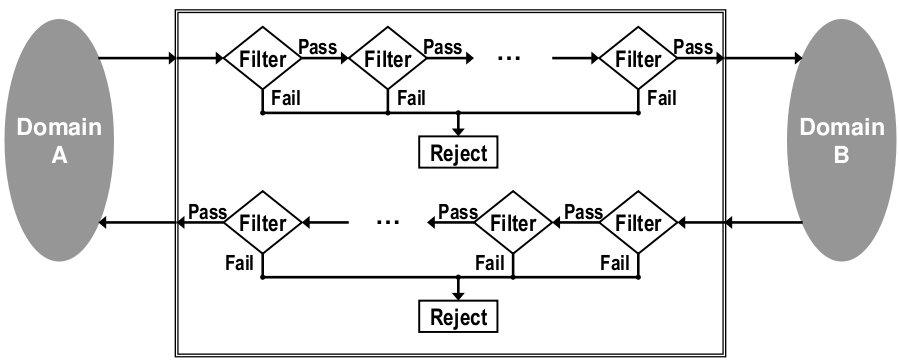
\includegraphics[width=3.4in]{nsa-legacy-arch}
\caption{NSA Legacy Model}
\label{fig:model:conceptual-model-nsa-legacy}
\end{figure}

\textit{Domain A} --- Private cloud managed by the Air Force
\newline
\textit{Domain B} --- A public operational network
\end{frame}

\begin{frame}[t]
\frametitle{Current Solutions --- NSA (SoA)}
Future cross-domain notional architecture \cite{proposal:nsa-arch}
\begin{figure}[!t]
\centering
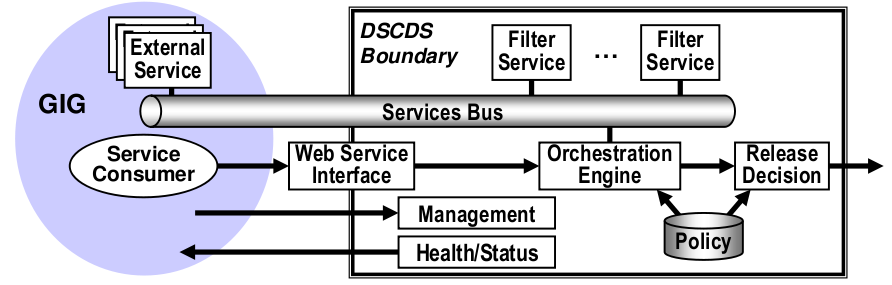
\includegraphics[width=3.4in]{nsa-arch}
\caption{NSA Service-Oriented Model}
\label{fig:model:conceptual-model-nsa}
\end{figure}

\textit{GiG} --- Global Information Grid; a large public cloud operated by the DoD
\newline
\textit{DSCDS} --- Distributed Service-oriented Cross Domain Solution
\end{frame}

\begin{frame}[t]
\frametitle{Current Solutions --- Raytheon}
Raytheon's notional architecture supporting cross-domain information flow \cite{proposal:raytheon-arch}:
\begin{figure}[!t]
\centering
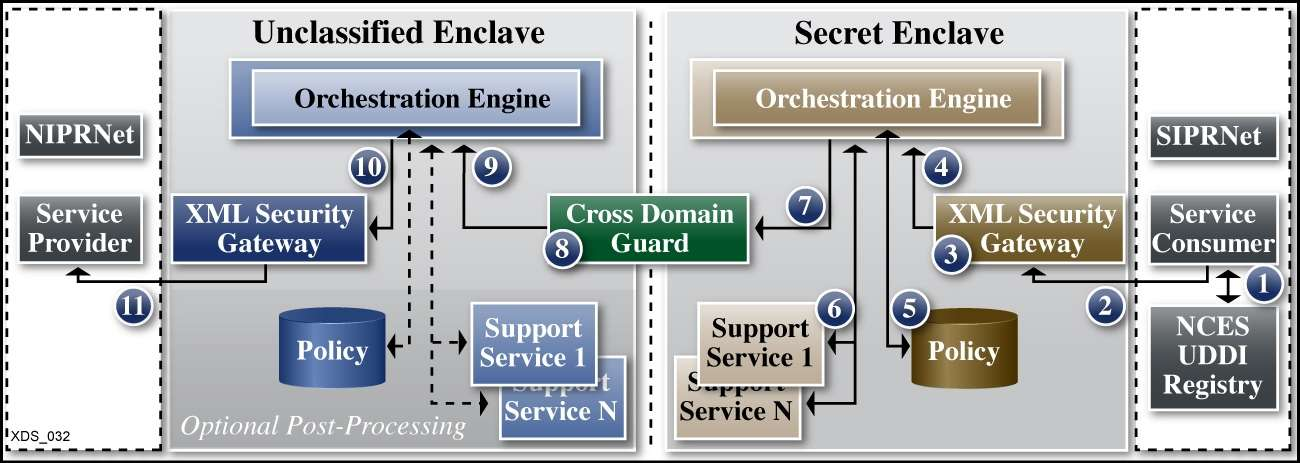
\includegraphics[width=3.4in]{raytheon-arch}
\caption{Raytheon Model}
\label{fig:model:conceptual-model-raytheon}
\end{figure}

\textit{...still uses a single perimeter guard...}
\end{frame}

\begin{frame}[t]
\frametitle{Current Solutions --- BAH}
{Booz$\mid$Allen$\mid$Hamilton} presented a service-centric cross domain solution in 2009 \cite{proposal:bah-arch}:
\begin{figure}[!t]
\centering
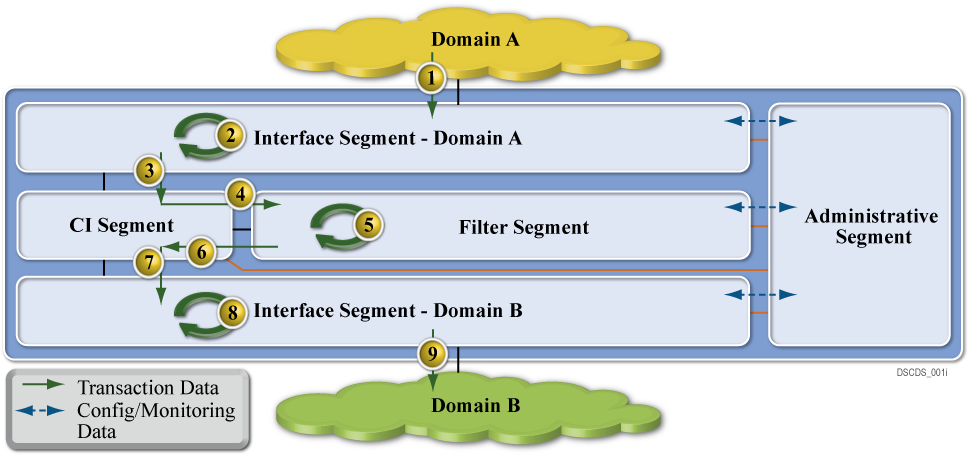
\includegraphics[width=3.4in]{bah-arch}
\caption{Booz|Allen|Hamilton Model}
\label{fig:model:conceptual-model-bah}
\end{figure}
\textit{...still uses a single perimeter guard (called a filter segment)...}
\end{frame}

\begin{frame}[t]
\frametitle{Future Solution}
Organizations are falling back on what they know in the scope of new problems.
\begin{figure}[!t]
\centering
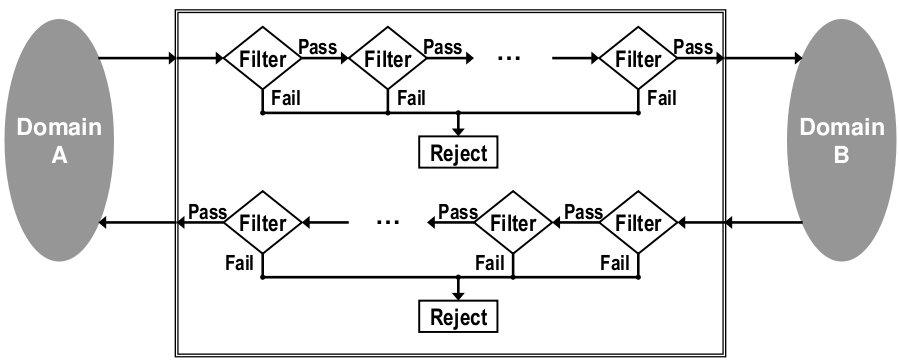
\includegraphics[width=3.4in]{nsa-legacy-arch}
\caption{NSA Legacy Model}
\label{fig:model:conceptual-model-nsa-legacy-II}
\end{figure}
Even though we know they don't work \cite{proposal:ron-ross}.
\end{frame}

%overlay:
%- Policy into network fabric
%- Multiple compartments on same physical network
%- Network can integrate cloud components securely
%- Provides security in depth
%
%traditional/guard:
%- Policy centralized single points of failure
%- Each physical network can only be at one compartment level
%- Use is tied to the physical network; no cloud integration possible
%- Boundary security only 
\begin{frame}
\frametitle{Characteristics of Current Solutions}
\begin{itemize}
\item<2-> \textit{Centralized Policy} --- They use centralized policy injection into communication flow.  Note that in each sample model, policy is \textit{only} evaluated at guard points.
\item<3-> \textit{Physical to Compartment Mapping} --- In each of these cases, users are only allowed to exchange one type of information per domain.  The physical domain systems are locked (by operational policy) to a single classification level limit.  Users cannot, for example, have \emph{Top Secret} material on a network accredited for \emph{Secret} material.
\item<4-> \textit{Perimeter Protection} --- The use of a single policy enforcement point at domain interconnects supplies a crunchy exterior to the creamy interior data filling.
\end{itemize}
\end{frame}

\begin{frame}
\frametitle{What's Wrong with Current Solutions?}
\begin{itemize}
\item<2-> \textit{Centralized Policy} --- A centralized policy enforcement system simplifies infrastructural attacks.  Adversaries know exactly where to focus efforts to compromise policy enforcement, lowering overall system trustworthiness and reliability. 
\item<3-> \textit{Physical to Compartment Mapping} --- The traditional model for multi-level security, enforced in this scheme, is that the network is classified at the level of the most sensitive data that transits it.  Ergo, those that have clearances at a level to view sensitive data are unable to view that data generally without extensive swivel-chair integration.
\item<4-> \textit{Perimeter Protection} --- Perimeter protection is a necessary but not sufficient security approach.  By itself, it doesn't work \cite{proposal:ron-ross}.
\end{itemize}
\end{frame}

\begin{frame}
\frametitle{Characteristics of Future Solutions}
\begin{itemize}
\item<2-> \textit{Decentralized Policy} --- Policy management is decentralized and integrated within the fabric of the system.  The system is both more secure and resilient as a result, better able to control information and operate under stressful conditions.
\item<3-> \textit{Infrastructure Reuse} --- Multi-tenancy can lower costs and increase reliability and is furthermore a common attribute of cloud systems.  An appropriately secured system facilitates integration of computing resources into multi-tenant environments.
\end{itemize}
\end{frame}

\begin{frame}
\frametitle{Characteristics of Future Solutions}
\begin{itemize}
\item<2-> \textit{Cloud Integration} --- The ability to handle multi-tenant environments and to reliably secure both data at rest and data in motion leads to computational environments deployable in cloud systems.
\item<3-> \textit{Security in Depth} --- Systems must operate under \textit{all} conditions, including when they are under attack or compromise \cite{proposal:ron-ross}.  Ergo, they must provide protection to sensitive data in depth.
\end{itemize}
\end{frame}

\section{System Architecture}
\begin{frame}
\frametitle{System Architecture}
What would this kind of overlay system look like?
\pause
\begin{itemize}
\item \textit{Meta-Model}
\pause
\item \textit{Non-Hierarchical Overlays}
\pause
\item \textit{Hierarchical Overlays}
\pause
\item \textit{Ontologies and Taxonomies}
\end{itemize}
\
\newline
\newline
\pause
\textit{...and what would the migration path to these systems look like?}
\end{frame}

\begin{frame}[t]
\frametitle{System Architecture - Level $\phi$}
\begin{figure}[!t]
\centering
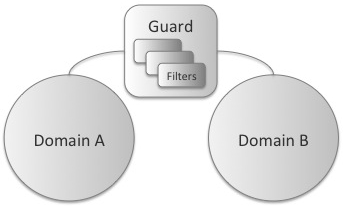
\includegraphics[width=2in]{model-phi-crop}
\label{fig:model:phi}
\end{figure}
This is a baseline cross-domain solution.  It is filter based and does not have any external  policy sources.  These are primarily:
\pause
\newline
\begin{itemize}
\item \textit{Filter-centric} --- They use content filters of some sort against submitted information.
\pause
\item \textit{Blacklist-oriented} --- They use hard-wired blacklists to filter and redact.
\end{itemize}
\end{frame}

\begin{frame}[t]
\frametitle{System Architecture - Level $\alpha$}
\begin{figure}[!t]
\centering
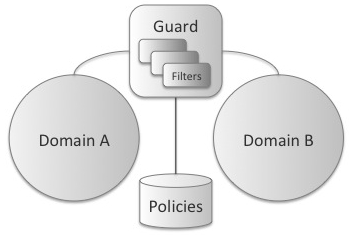
\includegraphics[width=2in]{model-alpha-crop}
\label{fig:model:alpha}
\end{figure}
This is a more advanced cross-domain solution featuring distributed policy management.  Characteristics include:
\pause
\newline
\begin{itemize}
\item {Generalized Control} --- No longer required to use fixed blacklist-centric solutions, these kinds of systems process policies defined over a more general ontology \footnote{Ontological impedance now a problem}.
\end{itemize}
\end{frame}

\begin{frame}[t]
\frametitle{System Architecture - Level $\beta$}
\begin{figure}[!t]
\centering
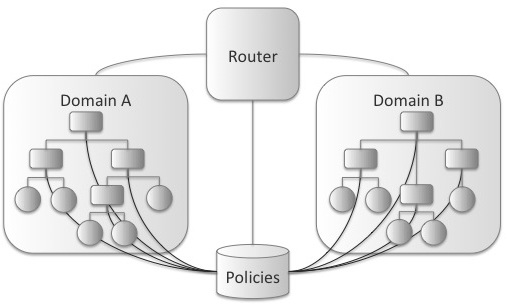
\includegraphics[width=2in]{model-beta-crop}
\label{fig:model:beta}
\end{figure}
We are beginning to inject usage management into the fabric of the network, linking content routing elements to policy information \footnote{Not really applicable to pure non-hierarchical systems}.
\newline
\pause
\begin{itemize}
\item \textit{Content-based Routing} --- We can start to implement content based routing at this point with available policy information.
\pause
\item \textit{Dynamic Context} --- We can also start to take advantage of changing network context with respect to routing data.
\end{itemize}
\end{frame}

\begin{frame}[t]
\frametitle{System Architecture - Level $\gamma$}
\begin{figure}[!t]
\centering
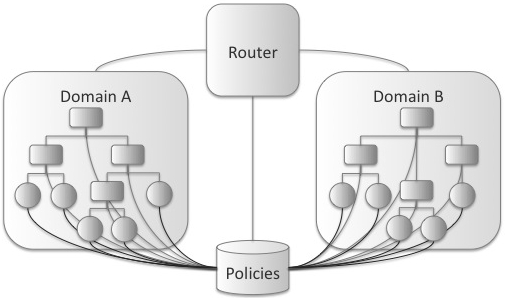
\includegraphics[width=2in]{model-gamma-crop}
\label{fig:model:gamma}
\end{figure}
We now are injecting usage management into every content node within the system.  This gives us:
\newline
\pause
\begin{itemize}
\item \textit{Extensive Control} --- We can now effectively do things like \textit{rights retraction}.
\pause
\item \textit{Pervasive Usage Management } --- We have content monitoring at all nodes of the content network.
\end{itemize}
\end{frame}

\begin{frame}[t]
\frametitle{System Architecture - Level $\delta$}
Here, we introduce the concept of a \textit{Smart License}:
\begin{itemize}
\pause
\item \textit{Mobile} --- Licenses are small programs that move along the overlay and are run at various policy enforcement points \cite{proposal:rfc3198}
\pause
\item \textit{Integrated} --- Content, Policies, Usage Management Mechanism all packaged in Smart License
\pause
\item \textit{Contained} --- Content and Policies are never exposed, all access to content is through specific interfaces
\end{itemize}
\pause
\begin{columns}[t]
\column{.5\textwidth}
\textit{Advantages}
\pause
\newline
\newline
Potentially more \textbf{secure} for content, provides finest-grained \textbf{control}; \textbf{simpler} routers and nodes
\column{.5\textwidth}
\textit{Disadvantages}
\pause
\newline
\newline
Mobile code requires \textbf{uniform execution environments}, which have their own \textbf{security} problems; \textbf{complex} license
\end{columns}
\end{frame}

\begin{frame}
\frametitle{Costs and Benefits}
So we have integrated usage management into a content network taking a very information-centric perspective.  At what cost?
\newline
\pause
\begin{columns}[t]
\column{.5\textwidth}
\textit{Costs}
\pause
\newline
\newline
Increasing \textbf{attack surface}; all these policy evaluation and injection points are nifty avenues for exploitation
\pause
\newline
\newline
Increasing \textbf{complexity}; dynamic routing makes things more difficult and expensive to manage
\column{.5\textwidth}
\textit{Benefits}
\pause
\newline
\newline
Additional \textbf{control} over sensitive content; both how it is \textbf{used} and how it is \textbf{distributed}
\pause
\newline
\newline
The ability to dynamically apply \textbf{new security controls} to transmitted information based on context (e.g. increase the strength of encryption)
\end{columns}
\end{frame}
\section{Progress}

\begin{frame}
\frametitle{Initial Prototype}
\begin{figure}
\centering
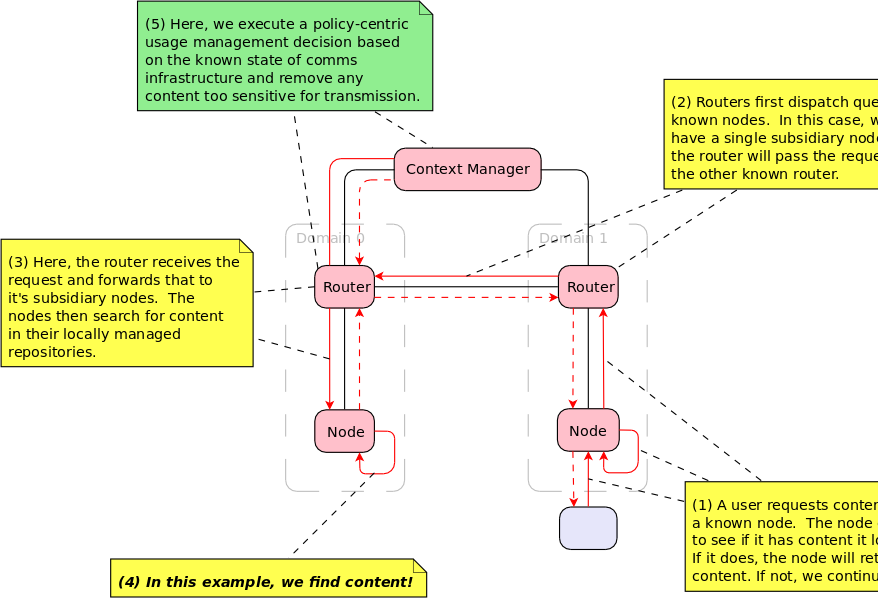
\includegraphics[width=4in]{cross-domain-prototype}
\label{fig:implementation:prototype}
\end{figure}
\end{frame}

\begin{frame}
\frametitle{Current Work}
We're currently extending the local simulation to a distributed content system.  The environment we're using consists of roughly 40 nodes distributed over Rackspace (using Rackspace Servers), Amazon (using EC2), and our local Eucalyptus installation.  We will use Heroku as well (We're deliberately building networks over providers and mixing IAAS and PAAS).
\newline
\pause
\begin{itemize}
\item \textit{Ruby} --- We use Ruby and the Ruby runtime as our base runtime engine.  We use associated tools like RVM, Gem, and Bundler to manage our projects.
\pause
\item \textit{Sinatra} --- Sintara is a simple but powerful HTTP engine.
\pause
\item \textit{Capistrano} --- Capistrano simplifies deployment of software on large numbers of nodes.
\pause
\item \textit{YAML} --- YAML is a simple data serialization language.
\end{itemize}
\end{frame}

\begin{frame}[c]
\frametitle{Future Work}
We are in the process of configuring infrastructure to begin work with Openflow-enabled hardware.  We will use Ruby and Ruby tools in this environment as well, with the addition of Trema, a Ruby and C based environment for building Openflow controllers.
\end{frame}
\section{Conclusions}

\begin{frame}
\frametitle{Conclusions}
\begin{beamerboxesrounded}[shadow]{Contribution of Work}
The contribution of this work is a quantitative analysis of policy-centric overlay network options, associated taxonomies of use, and prototypical technology proofs-of-concept.
\end{beamerboxesrounded}
\begin{itemize}
\item \textit{Network Control Options} --- This includes various types networks and associated strengths and weaknesses addressing centralized and decentralized models.
\item \textit{Taxonomies of Use} --- Depending on the specific usage management requirements and context, different overlays have different applicability; this work will provide guidance on suitability; it will eventually lead to how to manage data flow within SDN-capable infrastructure.
\item \textit{Prototypical Technologies} --- Examples and proofs-of-concept will be required to appropriately analyze various architectural alternatives.
\end{itemize}
\end{frame}

\begin{frame}[c]
\begin{center}
\textbf{Questions? Comments?}
\end{center}
\end{frame}
\section{References}
\begin{frame}
\def\newblock{}
\tiny{
\bibliographystyle{abbrv}
\bibliography{bib/proposal}}
\end{frame}

\end{document}

